\chapter{公式、图像和表格}
\label{chap:example}

公式、图表和插图广泛使用于学位论文中,并且在正文内存在较多的交叉引用,对他们的高效处理也是\LaTeX{}的优势之一。公式、图表和插图在定义时的共同特点包含:定义中需要设定引用标签、设置图表名称。定义时,图表摆放位置并无要求,\LaTeX{}会根据文稿内容自动计算图表摆放位置,不会出现表格窜行的问题。

\section{公式与数学环境}

\subsection{公式及术语表}
\label{sec:eqn}

公式定义的内容包含在\verb|\begin{equation}|\verb|\end{equation}|之间。为方便,公式的编辑可以采用\textbf{在线的\LaTeX{}公式编辑器}(截至2023年,\href{https://www.latexlive.com/}{latexlive.com}可以视为一个不错的例子)。一般的\LaTeX{}编辑器如 TexStudio 也都会提供语法补全。

{\bf{实例1:}} 以下是L-B非稳态流动升力模型,公式引用为公式\ref{eqn:LBmodel}。该公式的术语列表见 表 \ref{tab:LB-parameters}。
\begin{equation}
 \label{eqn:LBmodel}
   C_{L}=C_{L0}+C_{L\alpha }\left ( \frac{1+\sqrt{X}}{2} \right )\alpha 
\end{equation}

\begin{lstlisting}[language={[LaTeX]TeX}, caption={L-B非稳态流动升力模型}]
\begin{equation}
 \label{eqn:LBmodel}
   C_{L}=C_{L0}+C_{L\alpha }\left ( \frac{1+\sqrt{X}}{2} \right )\alpha 
\end{equation}
\end{lstlisting}

\subsection{长公式排版}


《Math mode》里有举一个长公式排版的例子如下。《Math mode》有十分丰富实用的例子,感兴趣的同学可以参考一下。

\begin {multline}
  \frac {1}{2}\Delta (f_{ij}f^{ij})=
  2\left (\sum _{i<j}\chi _{ij}(\sigma _{i}-
    \sigma _{j}) ^{2}+ f^{ij}\nabla _{j}\nabla _{i}(\Delta f)+\right .\\
  \left .+\nabla _{k}f_{ij}\nabla ^{k}f^{ij}+
    f^{ij}f^{k}\left [2\nabla _{i}R_{jk}-
      \nabla _{k}R_{ij}\right ]\vphantom {\sum _{i<j}}\right )
\end{multline}

\begin{lstlisting}[language={[LaTeX]TeX}, caption={长公式排版}]
\begin {multline}
  \frac {1}{2}\Delta(f_{ij}f^{ij})=
  2\left(\sum_{i<j}\chi_{ij}(\sigma_{i}-
    \sigma_{j}) ^{2}+ f^{ij}\nabla_{j}\nabla_{i}(\Delta f)+\right.\\
  \left.+\nabla_{k}f_{ij}\nabla ^{k}f^{ij}+
    f^{ij}f^{k}\left [2\nabla_{i}R_{jk}-
      \nabla_{k}R_{ij}\right]\vphantom{\sum_{i<j}}\right )
\end{multline}
\end{lstlisting}

\subsection{定理环境}

在~bithesis.cls~中定义了丰富的定理\textbf{环境}
algo(算法),them(定理),lem(引理),prop(命题),cor(推论),defn(定义),conj(猜想),exmp(例),rem(注),case(情形),amsmath还提供了一个proof(证明)的环境。
这里举一个``定理''和``证明''的例子。
\begin{them}[留数定理]
\label{thm:res}
  假设$U$是复平面上的一个单连通开子集,$a_1,\ldots,a_n$是复平面上有限个点,$f$是定义在$U\backslash \{a_1,\ldots,a_n\}$上的全纯函数,
  如果$\gamma$是一条把$a_1,\ldots,a_n$包围起来的可求长曲线,但不经过任何一个$a_k$,并且其起点与终点重合,那么:

  \begin{equation}
    \label{eq:res}
    \ointop_{\gamma}f(z)\,\mathrm{d}z = 2\uppi\mathbf{i}\sum^n_{k=1}\mathrm{I}(\gamma,a_k)\mathrm{Res}(f,a_k)
  \end{equation}

  如果$\gamma$是若尔当曲线,那么$\mathrm{I}(\gamma, a_k)=1$,因此:

  \begin{equation}
    \label{eq:resthm}
    \ointop_{\gamma}f(z)\,\mathrm{d}z = 2\uppi\mathbf{i}\sum^n_{k=1}\mathrm{Res}(f,a_k)
  \end{equation}

  在这里,$\mathrm{Res}(f, a_k)$表示$f$在点$a_k$的留数,$\mathrm{I}(\gamma,a_k)$表示$\gamma$关于点$a_k$的卷绕数。
  卷绕数是一个整数,它描述了曲线$\gamma$绕过点$a_k$的次数。如果$\gamma$依逆时针方向绕着$a_k$移动,卷绕数就是一个正数,
  如果$\gamma$根本不绕过$a_k$,卷绕数就是零。

  定理\ref{thm:res}的证明。
  
  \begin{proof}
    首先,由……

    其次,……

    所以……
  \end{proof}
  
\end{them}

\begin{lstlisting}[language={[LaTeX]TeX}, caption={定理环境}]
\begin{them}[留数定理]
假设$U$是复平面上的一个单连通开子集...... 
\end{them}
\end{lstlisting}

\begin{lstlisting}[language={[LaTeX]TeX}, caption={证明环境}]
  \begin{proof}
    首先,由……
    其次,……
    所以……
  \end{proof}
\end{lstlisting}

上面的公式例子中,有一些细节需要注意。微分号d应该使用``直立体'',也就是用mathrm包围起来。
并且,微分号和被积函数之间应该有一段小间隔,可以插入\verb+\,+得到,也可使用\verb+\dif+来输入微分符号。
斜体的$d$通常只作为一般变量。
i,j作为虚数单位时,也应该使用``直立体'',为了明显,还加上了粗体,例如\verb+\mathbf{i}+。斜体$i,j$通常用作表示``序号''。
其他字母在表示常量时,也推荐使用``直立体'',譬如,圆周率$\uppi$(需要upgreek宏包),自然对数的底$\mathrm{e}$。


\section{向文档中插入图像}
\label{sec:insertimage}

\subsection{支持的图片格式}
\label{sec:imageformat}

\LaTeX~ 可以很方便地插入~PDF、EPS、PNG、JPG~格式的图片。

在学位论文中,插图地使用简单地分为两类:单列图片和多列图片。图片的格式包含*.jpg、*.eps、*.pdf,既可以是位图也可以是矢量图,在插入图片时可以定义其高度和宽度。

最基本的图片插入示例可见图\ref{fig:diagram},其代码如\ref{demo-figure1}所示。

其中\verb+\centering+表示图片居中,\verb+\includegraphics[...]{...}+导入图片并制定图片大小,\verb+\caption{}+指定图片标题,而\verb+\label{...}+为图片加上引用标签。

\begin{figure}
 \centering
 \includegraphics[width=0.75\textwidth]{example-image}
 \caption{单张图片插入的基本示例}\label{fig:diagram}
\end{figure}

\begin{lstlisting}[language={[LaTeX]TeX}, caption={示例插图代码}, label=demo-figure1]
\begin{figure}
 \centering
 \includegraphics[width=0.75\textwidth]{example-image}
 \caption{单张图片插入的基本示例}\label{fig:diagram}
\end{figure}
\end{lstlisting}

插入两幅图片的例子如\ref{fig:png-jpg}所示。
这两个水平并列放置的图共享一个``图标题''(table caption),没有各自的小标题。

\begin{figure}
  \centering
  \includegraphics[width=0.35\textwidth]{example-image-a}
  \hspace{1cm}
  \includegraphics[width=0.35\textwidth]{example-image-b}
  \caption{水平并列放置图片的基本示例}
  \label{fig:png-jpg}
\end{figure}

\begin{lstlisting}[language={[LaTeX]TeX}, caption={插入PNG/JPG}]
\begin{figure}
  \centering
  \includegraphics[width=0.35\textwidth]{example-image-a}
  \hspace{1cm}
  \includegraphics[width=0.35\textwidth]{example-image-b}
  \caption{水平并列放置图片的基本示例}
  \label{fig:png-jpg}
\end{figure}
\end{lstlisting}

更多关于~\LaTeX~ 插图的例子可以参考《~\LaTeX~插图指南》。

\subsection{长标题的换行}
\label{sec:longcaption}

图\ref{fig:longcaptionbad}和图\ref{fig:longcaptiongood}都有比较长图标题,通过对比发现,图\ref{fig:longcaptiongood}的换行效果更好一些。
其中使用了minipage环境来限制整个浮动题的宽度。

不过在实际使用中,你可以根据排版的整体效果来自行决定。

\begin{figure}
 \centering
 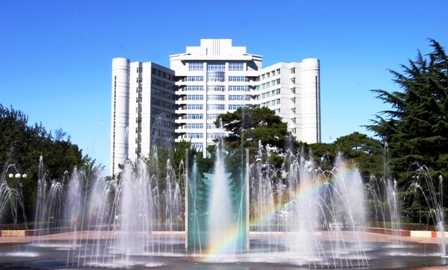
\includegraphics[width=10cm]{figures/pic1}
 \caption{BIT是我国历史最悠久的高等学府之一,是教育部直属、工信部共建的全国重点大学,985,211}
 \label{fig:longcaptionbad}
\end{figure}

\begin{figure}
  \centering
  \begin{minipage}[b]{0.6\textwidth}
  \centering
  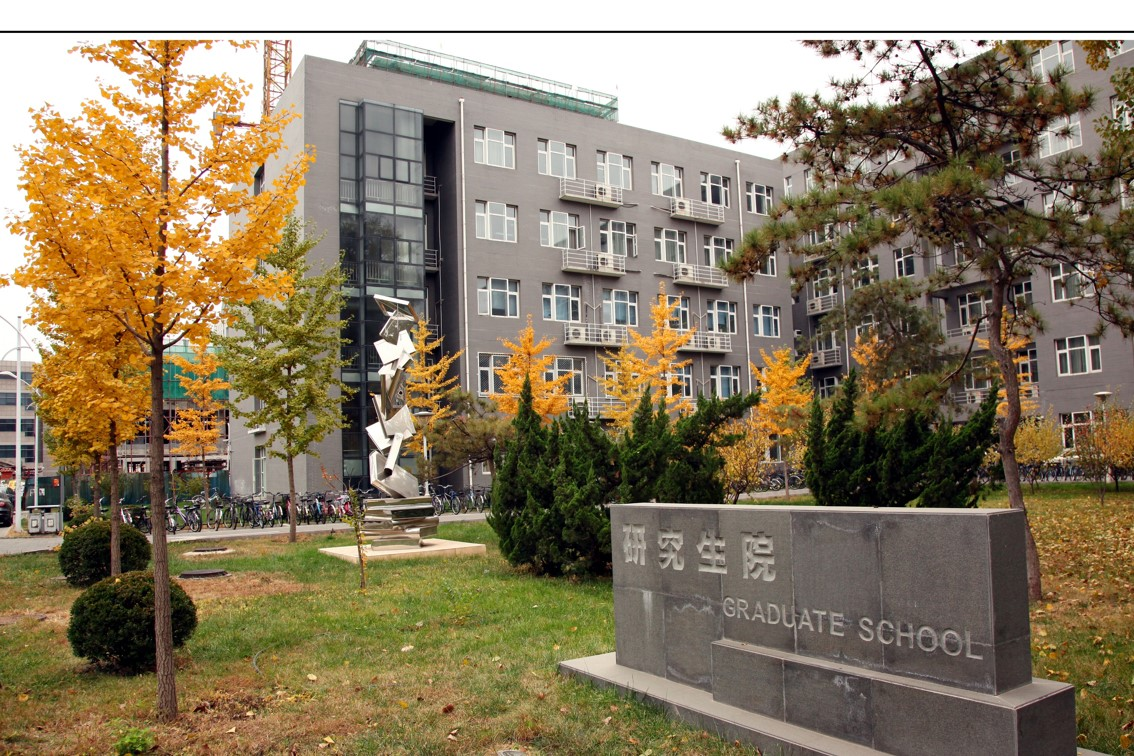
\includegraphics[width=10cm]{figures/pic2}
  \caption{BIT是我国历史最悠久的高等学府之一,是教育部直属、工信部共建的全国重点大学,985,211}
  \label{fig:longcaptiongood}
   \end{minipage}     
\end{figure}

\begin{lstlisting}[language={[LaTeX]TeX}, caption={长标题的换行}]
\begin{figure}
 \centering
 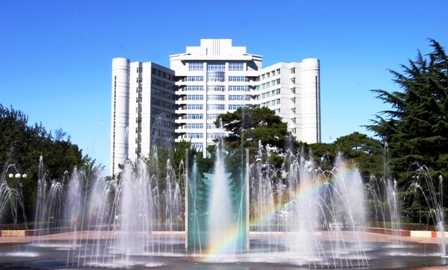
\includegraphics[width=10cm]{figures/pic1}
 \caption{BIT是我国历史最悠久的高等学府之一,是教育部直属、工信部共建的全国重点大学,985,211}
 \label{fig:longcaptionbad}
\end{figure}

\begin{figure}
  \centering
  \begin{minipage}[b]{0.6\textwidth}
  \centering
  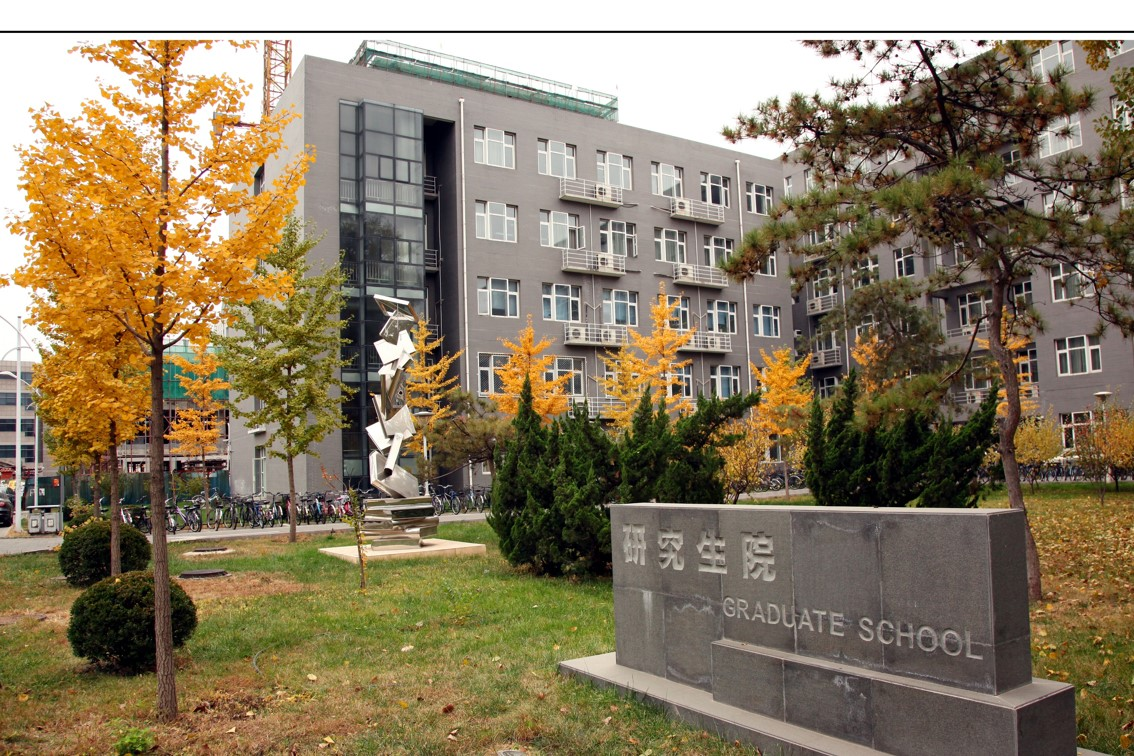
\includegraphics[width=10cm]{figures/pic2}
  \caption{BIT是我国历史最悠久的高等学府之一,是教育部直属、工信部共建的全国重点大学,985,211}
  \label{fig:longcaptiongood}
   \end{minipage}     
\end{figure}
\end{lstlisting}
  
\section{表格的例子}
\label{sec:tab}

表格的定义和引用就不多做介绍,表格内容包含在\textbackslash begin\{table\}和\textbackslash end\{table\}之间。这里给出一些表格的例子。

\textbf{\href{https://www.tablesgenerator.com/}{Tables Generator}可以用于在线生成表格}

先以模板示例中第一章的表\ref{tab:category}为例,插入代码为\ref{demo-table1}所示。

\begin{lstlisting}[language={[LaTeX]TeX}, caption={示例插表代码}, label=demo-table1]
\begin{table}
  \centering
  \caption{水系聚氨酯分类} \label{tab:category}
  \begin{tabular*}{0.9\textwidth}{@{\extracolsep{\fill}}cccc}
  \toprule
    类别			&水溶型		&胶体分散型		&乳液型 \\
  \midrule
    状态			&溶解$\sim$胶束	&分散		&白浊 \\
    外观			&水溶型		&胶体分散型		&乳液型 \\
    粒径$/\mu m$	&$<0.001$		&$0.001-0.1$		&$>0.1$ \\
    重均分子量	&$1000\sim 10000$	&数千$\sim 20万$ &$>5000$ \\
  \bottomrule
  \end{tabular*}
\end{table}
\end{lstlisting}

\begin{table}
  \centering
  \caption{模板示例中第一章的表一} \label{tab:category}
  \begin{tabular*}{0.9\textwidth}{@{\extracolsep{\fill}}cccc}
  \toprule
    类别			&水溶型		&胶体分散型		&乳液型 \\
  \midrule
    状态			&溶解$\sim$胶束	&分散		&白浊 \\
    外观			&水溶型		&胶体分散型		&乳液型 \\
    粒径$/\mu m$	&$<0.001$		&$0.001-0.1$		&$>0.1$ \\
    重均分子量	&$1000\sim 10000$	&数千$\sim 20$万 &$>5000$ \\
  \bottomrule
  \end{tabular*}
\end{table}

另举一个两列的表格例子(表\ref{tab:LB-parameters}以及代码\ref{demo-table2})。

\begin{table}              % no placement specified: defaults to here, top, bottom, page
\centering
 \begin{center}
  \caption{L-B模型中参数的物理意义}
  \label{tab:LB-parameters}
  \begin{tabular}{cl}
      \toprule
       Parameters & Physical meaning       \\
      \midrule   % \hline
       $C_{L\alpha}$ & Lift curve slope \\
       $a_{1}$ & Controls the shape of the stall curve \\
       $\alpha^{\star}$ & The break point at which $X=0.5$ \\
       $\tau_{1}$ & Represents the tendency of the model to track the static curve \\
       $\tau_{2}$ & Gives the model lift overshoot \\
      \bottomrule
  \end{tabular}
 \end{center}
\end{table}

\begin{lstlisting}[language={[LaTeX]TeX}, caption={插入表格\ref{tab:LB-parameters}}, label=demo-table2]
\begin{table}
\centering
 \begin{center}
  \caption{L-B模型中参数的物理意义}
  \begin{tabular}{cl}
      \toprule
       Parameters & Physical meaning       \\
      \midrule 
       $C_{L\alpha}$ & Lift curve slope \\
       $a_{1}$ & Controls the shape of the stall curve \\
       $\alpha^{\star}$ & The break point at which $X=0.5$ \\
       $\tau_{1}$ & Represents the tendency of the model to track the static curve \\
       $\tau_{2}$ & Gives the model lift overshoot \\
      \bottomrule
  \end{tabular}
 \end{center}
\end{table}
\end{lstlisting}

再给出一些表格的例子,如表\ref{tab:firstone}、代码\ref{demo-table3}所示。

\begin{table}
  \centering
  \caption{一个标准的三线表格}
  \label{tab:firstone}
  \begin{tabular}{@{}llr@{}} \toprule
    \multicolumn{2}{c}{Item} \\ \cmidrule(r){1-2}
    Animal & Description & Price (\$)\\ \midrule
    Gnat & per gram & 13.65 \\
    & each & 0.01 \\
    Gnu & stuffed & 92.50 \\
    Emu & stuffed & 33.33 \\
    Armadillo & frozen & 8.99 \\ \bottomrule
  \end{tabular}
\end{table}

\begin{lstlisting}[language={[LaTeX]TeX}, caption={三线表格}, label=demo-table3]
\begin{table}
  \centering
  \caption{一个标准的三线表格}
  \label{tab:firstone}
  \begin{tabular}{@{}llr@{}} \toprule
    \multicolumn{2}{c}{Item} \\ \cmidrule(r){1-2}
    Animal & Description & Price (\$)\\ \midrule
    Gnat & per gram & 13.65 \\
    & each & 0.01 \\
    Gnu & stuffed & 92.50 \\
    Emu & stuffed & 33.33 \\
    Armadillo & frozen & 8.99 \\ \bottomrule
  \end{tabular}
\end{table}
\end{lstlisting}


\section{参考文献管理}
\label{sec:reference}
\subsection{将参考文献的内容与表现分离}

\BIThesis{}论文模板使用 \href{https://www.ctan.org/pkg/biblatex}{BibLaTeX} 处理参考文献。它的出现让我们摆脱手写参考文献条目
的麻烦。
当然,使用者也可以手动编参考文献item,直接插入文档中。但是,有BibLaTeX帮助,处理起参考文献更为简单。

参考文献的具体内容就是reference文件夹下的\textit{main.bib},
参考文献的元数据(名称、作者、出处等)以一定的格式保存在这些纯文本文件中。
.bib文件也可以理解为参考文献的``数据库'',正文中所有引用的参考文件条目都会从这些文件中``析出''。
控制参考文献条目``表现形式''(格式)的代码通过 main.tex 中的 \\ \verb|\usepackage[style=gb7714-2015,...]{biblatex}| 引入。
按照学校要求,本模板使用的是国标GB/T 7714风格的参考文献析出格式(最新版本)。

.bib数据库中的参考文献条目可以手动编写,也可以在Google的学术搜索中找到。
各大数据库也支持将参考文献信息导出为.bib,省时省力。
以Google学术搜索为例:在搜索结果中,选择``引用''、``BibTeX''的连接,
点击后浏览器会打开新的标签页,出现类似代码\ref{googlescholar}所示的内容。

\begin{lstlisting}[caption={从Google Scholar找到的,但并不规范的.bib条目}, label=googlescholar, float, escapeinside="", numbers=none]
@article{张玲2000信用风险评估方法发展趋势,
  title={信用风险评估方法发展趋势},
  author={张玲 and 张佳林},
  journal={预测},
  volume={19},
  number={4},
  pages={72--75},
  year={2000}
}
\end{lstlisting}

\subsection{在正文中引用参考文献}

\textit{如果想要按照章节分别管理参考文献,可以详见 biblatex中关于refsection 的部分。简单来说,就是使用 refsection 包裹一个章节的全部内容即可。但由于我校论文要求并非采用章节管理,因此不做赘述。}

正文中引用参考文献时\cite{Jiang2005Size},用\verb+\cite{key1,key2,key3...}+可以产生“上标引用的参考文献”,
如\cite{Meta_CN,chen2007act,DPMG}。
使用\verb+\parencite{key1,key2,key3...}+则可以产生水平引用的参考文献,例如\parencite{JohnD,zhubajie,IEEE-1363}。
请看下面的例子,将会穿插使用水平的和上标的参考文献:关于书的\parencite{Meta_CN,JohnD,IEEE-1363},关于期刊的\cite{chen2007act,chen2007ewi},
会议论文\cite{DPMG,kocher99,cnproceed},
硕士学位论文\cite{zhubajie,metamori2004},博士学位论文\cite{shaheshang,FistSystem01,bai2008},标准文件\cite{IEEE-1363},技术报告\cite{NPB2},电子文献\cite{xiaoyu2001, CHRISTINE1998}。

最后总结一些注意事项:
\begin{itemize}
\item  参考文献只有在正文中被引用了,才会在最后的参考文献列表中出现;
\item  参考文献``数据库文件''.bib是纯文本文件,请使用~UTF-8~编码,不要使用~GBK~编码;
\item  参考文献条目同样有“内容”和“表现形式”之分,这种可控性是BibLaTeX带来的。
\end{itemize}


\section{用~listings~插入源代码}

这里给使用~listings~宏包插入源代码的例子,这里是一段C代码。另外,listings宏包可以实现各种复杂、漂亮的效果,想要进一步学习的同学,可以参考《The Listings Package》。

{\color{blue}
\begin{enumerate}
\item[] ~\verb|\begin{lstlisting}[language={C}, caption={一段C源代码}]|
\item[] ~\verb|#include <stdio.h>| 
\item[] ~\verb|...|
\item[] ~\verb|\end{lstlisting}|
\end{enumerate}}


\begin{lstlisting}[language={C}, caption={一段C源代码}]
#include <stdio.h>
#include <unistd.h>
#include <sys/types.h>
#include <sys/wait.h>

int main() {
  pid_t pid;

  switch ((pid = fork())) {
  case -1:
    printf("fork failed\n");
    break;
  case 0:
    /* child calls exec */
    execl("/bin/ls", "ls", "-l", (char*)0);
    printf("execl failed\n");
    break;
  default:
    /* parent uses wait to suspend execution until child finishes */
    wait((int*)0);
    printf("is completed\n");
    break;
  }

  return 0;
}
\end{lstlisting}

再给出一个插入MATLAB代码的例子。

{\color{blue}
\begin{enumerate}
\item[] ~\verb|\begin{lstlisting}[language={matlab}, caption={一段MATLAB源代码}]|
\item[] ~\verb|function paper1| 
\item[] ~\verb|r=0.05;|
\item[] ~\verb|n=100;|
\item[] ~\verb|...|
\item[] ~\verb|\end{lstlisting}|
\end{enumerate}}

\begin{lstlisting}[language={matlab}, caption={一段MATLAB源代码}]
function paper1
r=0.05;
n=100;
T=1;
X=1;
v0=0.8;
sigma=sqrt(0.08);
deltat=T/n;
for i=1:n
    t(i)=i*deltat;
    w(i)=random('norm',0,t(i),1);
end
for i=1:n
    alpha(i)=0.39;
end
for i=1:n
    temp=0;
    for k=1:i
        temp=temp+alpha(k);
    end
    B(i)=exp(r*t(i));
    BB(i)=B(i)*exp(temp*deltat);
    BBB(i)=exp(-r*(T-t(i)));
end
for i=1:n
    s0(i)=X*BBB(i);
    v(i)=v0*exp((r-0.5*sigma^2)*t(i)+sigma*w(i));
    for j=i+1:n
        D=X*BBB(j);
        d1=(log(v(i)/D)+(r+sigma^2/2)*(t(j)-t(i)))/(sigma*sqrt(t(j)-t(i)));
        d2=d1-(sigma*sqrt(t(j)-t(i)));
        ppp(i,j)=D*exp(-r*(t(j)-t(i)))*(1-cdf('normal',d2,0,1))-v(i)*(1-cdf('n
ormal',d1,0,1));
    end
end
for i=1:n
    s1(i)=0;
    for j=i+1:n
        s1(i)=s1(i)+BB(j)^(-1)*alpha(j)*deltat*(X*BBB(j)-B(j)/B(i)*ppp(i,j));
    end
    s2(i)=0;
    for j=1:n
        s2(i)=s2(i)+alpha(j);
    end
    s2(i)=X*exp(-r*T-s2(i)*deltat);
    s(i)=BB(i)*(s1(i)+s2(i));
end
plot(s)
hold on;
plot(s0);
\end{lstlisting}
  
